\documentclass[10pt,a4paper]{article}
\usepackage[utf8]{inputenc}
\usepackage[spanish]{babel}
\usepackage{amsmath}
\usepackage{amsfonts}
\usepackage{amssymb}
\usepackage{graphics}
\usepackage{graphicx}
\usepackage[left=2cm,right=2cm,top=2cm,bottom=2cm]{geometry}
\usepackage{imakeidx}
\makeindex[columns=3, title=Alphabetical Index, intoc]
\usepackage{listings}
\usepackage{xcolor}
\usepackage{multicol}
\usepackage{changepage}
\usepackage{float}
\usepackage{cite}
\usepackage{url}
\usepackage[document]{ragged2e}

\definecolor{codegreen}{rgb}{0,0.6,0}
\definecolor{codegray}{rgb}{0.5,0.5,0.5}
\definecolor{codepurple}{rgb}{0.58,0,0.82}
\definecolor{backcolour}{rgb}{0.95,0.95,0.92}

\lstdefinestyle{mystyle}{
    backgroundcolor=\color{backcolour},
    commentstyle=\color{codegreen},
    keywordstyle=\color{magenta},
    numberstyle=\tiny\color{codegray},
    stringstyle=\color{codepurple},
    basicstyle=\ttfamily\footnotesize,
    breakatwhitespace=false,
    breaklines=true,
    captionpos=b,
    keepspaces=true,
    numbers=left,
    numbersep=5pt,
    showspaces=false,
    showstringspaces=false,
    showtabs=false,
    tabsize=3
}

\lstset{style=mystyle}

\title{Comunication and Signals}

\author{Escrito por: Adrian González Pardo}

\date{\today}

\newcommand\tab[1][1cm]{\hspace*{#1}}

\begin{document}
% Portada
%encabezado
\begin{center}
	\par\vspace{0.25cm}{
		Instituto Tecnológico de Massachusetts\\Departamento de Ingenieria Mecanica\\2.14 Análisis y diseño de sistemas de control de retroalimentación}
	\par\vspace{0.5cm}{
    \large\textbf{{Comprensión de polos y ceros}}
	}
\end{center}
%Contenido
\section{Sistemas de Polos y Ceros}
La función de transferencia provee una base para determinar características importantes de respuesta del sistema sin resolver la ecuación diferencial completa. Se define, la función de transferencia como una función racional con variable compleja $s=\sigma + j\omega$, como esta:
\begin{center}
  \begin{minipage}{0.5\textwidth}
    \begin{center}
      \[H(s)=\frac{b{\scriptscriptstyle m}s^m+b{\scriptscriptstyle m-1}s^{m-1}+\cdots+b{\scriptscriptstyle 1}s+b{\scriptscriptstyle 0}} {a{\scriptscriptstyle n}s^n+a{\scriptscriptstyle n-1}s^{n-1}+\cdots+a{\scriptscriptstyle 1}s+a{\scriptscriptstyle 0}}\]
    \end{center}

  \end{minipage}
  \begin{minipage}{0.9\textwidth}
    \begin{flushright}
        (1)
    \end{flushright}
  \end{minipage}
\end{center}
A menudo es conveniente factorizar en el numerador y denominador, y escribir la función de transferencia en terminos de esos factores:
\begin{center}
  \begin{center}
    \[H(s)=\frac{N(s)}{D(s)}=K\frac{(s-z{\scriptscriptstyle 1})(s-z{\scriptscriptstyle 2})\cdots(s-z{\scriptscriptstyle m-1})(s-z{\scriptscriptstyle m})}{(s-p{\scriptscriptstyle 1})(s-p{\scriptscriptstyle 2})\cdots(s-p{\scriptscriptstyle m-1})(s-p{\scriptscriptstyle m})}\]
  \end{center}
  \begin{minipage}{0.9\textwidth}
    \begin{flushright}
        (2)
    \end{flushright}
  \end{minipage}
\end{center}
donde el numerador y el denominador son polinomios, $N(s)$ y $D(s)$, contienen coeficientes reales definidos por el sistema de ecuaciones diferenciales y $K=\frac{b{\scriptscriptstyle m}}{a{\scriptscriptstyle n}}$. Como se escriben en la Ec. $(2)$ los $z{\scriptscriptstyle i}$'s son las raíces de la ecuación
\begin{center}
  \begin{center}
    $N(s)=0$
  \end{center}
  \begin{minipage}{0.9\textwidth}
    \begin{flushright}
        (3)
    \end{flushright}
  \end{minipage}
\end{center}
y son definidos por los ceros, y los $p{\scriptscriptstyle i}$'s son las raíces de las ecuaciones
\begin{center}
  \begin{center}
    $D(s)=0$
  \end{center}
  \begin{minipage}{0.9\textwidth}
    \begin{flushright}
        (4)
    \end{flushright}
  \end{minipage}
\end{center}
y estan definidos en el sistema como polos. En la Ec $(2)$ los fatores en el numerador y denominador son escritos cuando $s=z{\scriptscriptstyle i}$ el numerador $N(s) = 0$ y la función de transferencia desaparece, es decir,
\begin{center}
  \[\lim_{s \to z{\scriptscriptstyle i}}H(s) = 0\]
\end{center}
y es similar cuando $s=p{\scriptscriptstyle i}$ el polinomio denominador $D(s)=0$ y el valor de la función de transferencia se vuelve infinita,
\begin{center}
  \[\lim_{s \to p{\scriptscriptstyle i}}H(s) = +\infty\]
\end{center}
Todos los coeficientes de los polinomios $N(s)$ y $D(s)$ son reales, por lo tanto los polos y ceros deben ser puramente reales o aparecer en pares de complejos conjugados. En general los polos, para $p{\scriptscriptstyle i}= \sigma{\scriptscriptstyle i}$, o bien $p{\scriptscriptstyle i},p{\scriptscriptstyle i+1}=\sigma{\scriptscriptstyle i} \pm j\omega{\scriptscriptstyle i}$. La existencia de un solo polo complejo sin un polo conjugado correspondiente generaría coeficientes complejos en el polinomio $D(s)$. Similarmente, el sistema de ceros es real o aparece un par de complejos conjugados.
\clearpage
\begin{center}
  \begin{tabular}{p{16cm}}
  \hline
  Ejemplo\\
  Un sistema linear descrito por la ecuación diferencial\\
  \begin{center}
    \[\frac{d^{2}y}{dt^{2}}+5\frac{dy}{dt}+6y=2\frac{du}{dt}+u\]
  \end{center}
  Encontrar el sistema de polos y ceros.\\
  \textbf{Solución:} La función de transferencia de la ecuación diferencial es
  \begin{center}
    \[H(s)=\frac{2s+1}{s^{2}+5s+6}\]
  \end{center}
  \begin{minipage}{0.9\textwidth}
    \begin{flushright}
        (5)
    \end{flushright}
  \end{minipage}
  Que puede escribirse en forma factorizada
  \begin{center}
    \[H(s)=\frac{1}{2}\frac{s+\frac{1}{2}}{(s+3)(s+2)}\]\\
    \tab\hspace{0.7cm}\[=\frac{1}{2}\frac{s-(-\frac{1}{2})}{(s-(-3))(s-(-2))}\]
  \end{center}
  \begin{minipage}{0.9\textwidth}
    \begin{flushright}
        (6)
    \end{flushright}
  \end{minipage}
  \\Por lo tanto el sistema tiene un solo cero real en $s=-\frac{1}{2}$, y un par de polos reales en $s=-3$ y $s=-2$.\\
  \hline
  \end{tabular}
\end{center}
Los polos y ceros son propiedades de la función de transferencia, y por lo tanto en la ecuación diferencial describen la entrada-salida  del sistema dinámico. Juntos con la constante de ganancia $K$ caracterizan a la ecuación diferencial completamente, y proveen una descripción al sistema.
\begin{center}
  \begin{tabular}{p{16cm}}
    \hline
    Ejemplo\\
    Un sistema tiene un par de polos complejos conjugados $p{\scriptscriptstyle 1},p{\scriptscriptstyle 2} = -1 \pm j2$, un solo cero $z{\scriptscriptstyle 1}=-4$, y un factor de ganancia $K=3$. Encontrar la ecuación diferencial que representa el sistema.\\
    \textbf{Solución:} La función de transferencia es
    \begin{center}
      \[H(s)=K\frac{s-z}{(s-p{\scriptscriptstyle 1})(s-p{\scriptscriptstyle 2})}\]\\
      \[=3\frac{s-(-4)}{(s-(-1 + 2j))(s-(-1 - 2j))}\]\\
      \[=3\frac{s+4}{s^{2}+2s+5}\]
    \end{center}
    \begin{minipage}{0.9\textwidth}
      \begin{flushright}
          (7)
      \end{flushright}
    \end{minipage}
    \\y la ecuación diferencial es
    \begin{center}
      \[\frac{d^{2}y}{dt^{2}}+2\frac{dy}{dt}+5y=3\frac{du}{dt}+12u\]
    \end{center}
    \begin{minipage}{0.9\textwidth}
      \begin{flushright}
          (8)
      \end{flushright}
    \end{minipage}
    \\
    \hline
  \end{tabular}
\end{center}
\clearpage
\begin{center}
  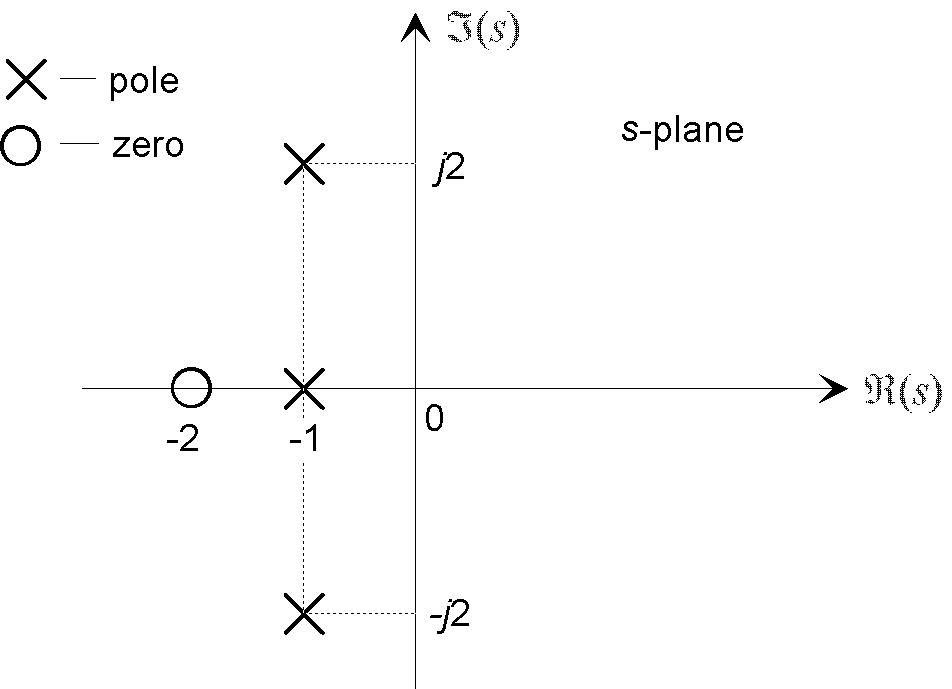
\includegraphics[scale=0.25]{img/poleAndZeros1.png}
\end{center}
\textit{Figura 1: El trazo polo-cero  para un sistema típico de tercer orden con un polo real y un par de polos complejo conjugados, y un cero real}
\subsection{Trazo del polo-cero}
Un sistema se caracteriza por sus polos y ceros en el sentido que estos permiten reconstruir por la entrada/salida de la ecuación diferencial. En general, los polos y ceros de la función de transferencia pueden ser complejos, y el sistema dinámico puede ser representado grafícamente tranzando sus localizaciones en el $plano-s $ $complejo$, cuyos ejes representan las partes real e imaginaria de la variable compleja $s$. Tales trazos son conocidos como trazos o graficos de polos-ceros. Es usual marcar la localización de un cero por un circulo ($\circ$) y la localización de un polo por una cruz ($\times$). La localización de los polos y ceros provee información cualitativa sobre las características de respuesta del sistema. Algunos programas de computadoras son utiles en la determinación de polos y ceros de un sistema desde una función de transferencia o las ecuaciones de estado del sistema [8]. La \textit{Figura 1} es un ejemplo de un grafíco de polo-cero de un sistema de tercer orden con un cero real, un polo real y un par de polos complejos conjugados, esto es:
\begin{center}
  \[H(s)=\frac{3s+6}{s^{3}+3s^{2}+7s+5}=3\frac{s-(-2)}{(s-(-1))(s-(-1-2j))(s-(-1+2j))}\]
\end{center}
\subsection{Polos del sistema y la respuesta homogénea }
Debido a la función de transferencia representa completamente una ecuación diferencial del sistema, sus polos y ceros definen efectivamente la respuesta del sistema. En particular el sistema directo de polos define los componentes en una respuesta homogénea. La respuesta no forzada de un sistema SISO (Single Input / Single Output)(Una Entrada / Una Salida) lineal a un conjunto de condiciones iniciales es
\begin{center}
  \begin{center}
    \[y{\scriptscriptstyle h}(t)=\sum_{i=1}^n C{\scriptscriptstyle i}e^{\lambda{\scriptscriptstyle i}t}\]
  \end{center}
  \begin{minipage}{0.9\textwidth}
    \begin{flushright}
        (9)
    \end{flushright}
  \end{minipage}
\end{center}
donde las constantes $C{\scriptscriptstyle i}$ se determinan a partir del conjunto de condiciones iniciales y los exponentes $\lambda{\scriptscriptstyle i}$ son las raíces de la ecuación característica o los eigenvalores del sistema. La ecuación característica es
\begin{center}
  \begin{center}
    \[D(s)= a{\scriptscriptstyle n}s^{n}+a{\scriptscriptstyle n-1}s^{n-1}+\cdots+a{\scriptscriptstyle 0}=0\]
  \end{center}
  \begin{minipage}{0.9\textwidth}
    \begin{flushright}
        (10)
    \end{flushright}
  \end{minipage}
\end{center}
y estas raíces son los polos del sistema, esas son $\lambda{\scriptscriptstyle i}=p{\scriptscriptstyle i}$, lo que lleva a la siguiente importante relación:
\clearpage
\begin{center}
  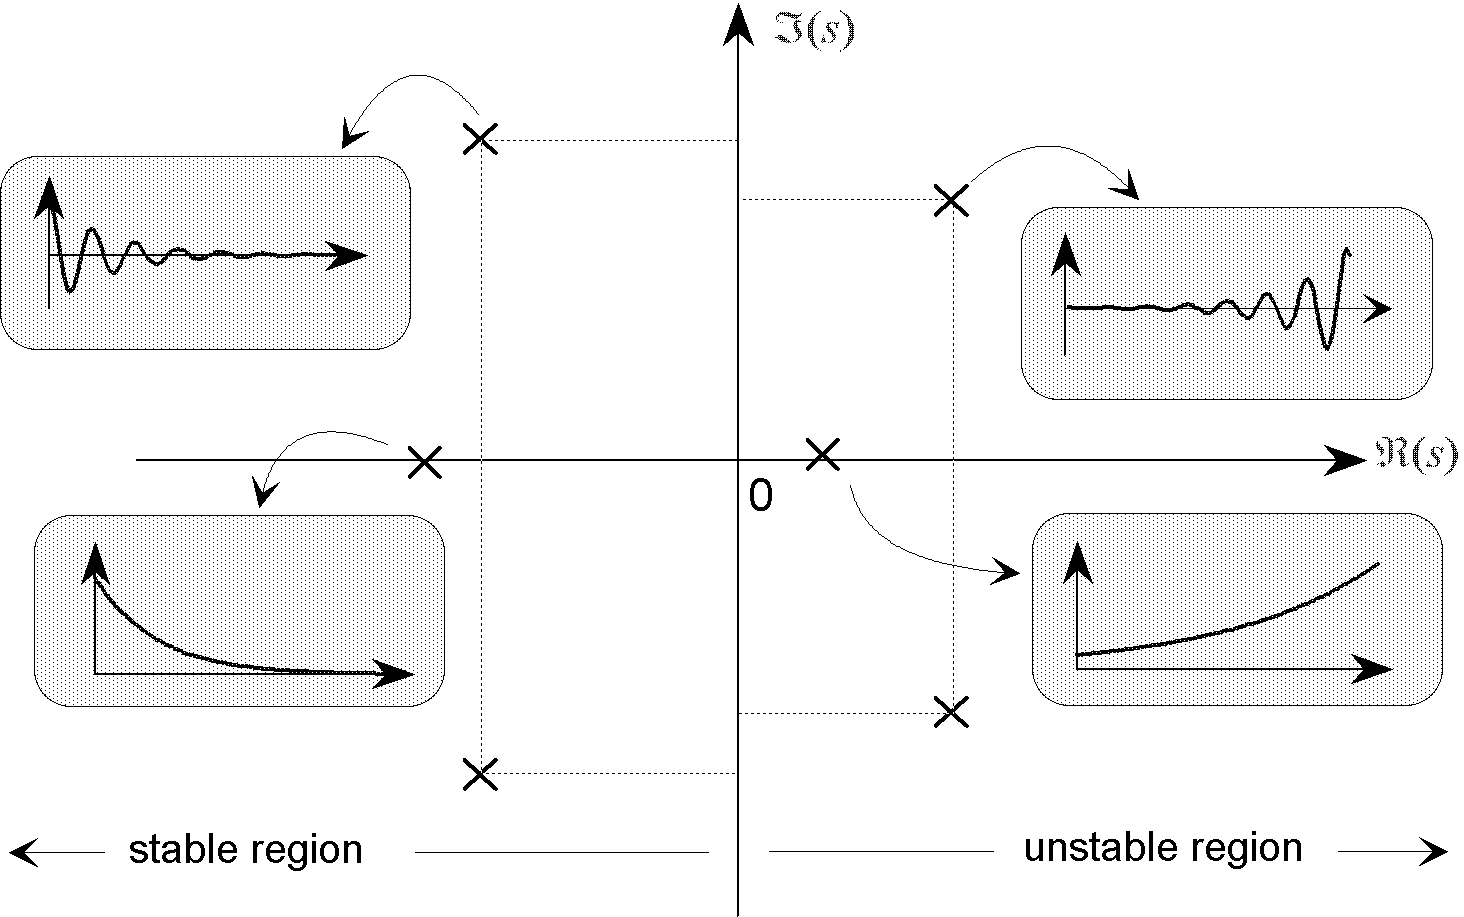
\includegraphics[scale=0.2]{img/grafica1.png}
\end{center}
\textit{Figura 2: Las especificaciones de la forma de los componentes de la respuesta homogénea a partir de la localización de polos en el grafíco de polos-ceros}
\begin{center}
  \begin{tabular}{p{14cm}}
    La función de transferencia de polos son las raices de la ecuación característica, y tambien los eigenvalores del sitema matricial $\mathbf{A}$\\
  \end{tabular}
\end{center}
Por lo tanto, la respuesta homogénea puede ser escrita
\begin{center}
  \begin{center}
    \[y{\scriptscriptstyle h}(t)=\sum_{i=1}^n C{\scriptscriptstyle i}e^{p{\scriptscriptstyle i}t}\]
  \end{center}
  \begin{minipage}{0.9\textwidth}
    \begin{flushright}
        (11)
    \end{flushright}
  \end{minipage}
\end{center}
Por lo tanto, la localización de los polos en el plano-s define los n componentes de la respuesta homogénea que se describe a continuación:
\begin{enumerate}
  \item Un polo real $p{\scriptscriptstyle i}=-\sigma$ en la mitad izquierda del plano-s define un componente de descomposición exponencial, $Ce^{-\sigma t}$, en la respuesta homogénea. El rango de descomposición se determina por la localización del polo; polos lejos del origen en la mitad izquierda del plano corresponden a componentes que se descomponen rapidamente, mientras que los polos más cercanos al origen corresponden a una descomposición con lentitud.
  \item Un polo en el origen $p{\scriptscriptstyle 0}$ define un componente que es constante en su amplitud y definido por las condiciones iniciales.
  \item Un polo real en la mitad derecha del plano corresponde a un componente de crecimiento exponencial $Ce^{\sigma t}$ en la respuesta homogénea; Esto define un sistema que es inestable.
  \item Un par de complejos conjugados $\sigma \pm j\omega$ en la mitad izquierda del plano-s combina un componente que genera una respuesta que se descompone sinusoidalmente de la forma $Ae^{-\sigma t}\sin(\omega t + \phi)$ donde $A$ y $\phi$ estan determinadas por las condiciones iniciales. El rango de descomposición es especificado por $\sigma$; la frecuencia de oscilación es determinada por $\omega$.
  \item Un par de polos imaginarios, polos que encuentran en el eje imaginario, $\pm j\omega$ genera un componente oscilador con la constante de amplitud es determinada por las condiciones iniciales
  \item Un par de polos complejos en la mitad derecha del plano genera un componente de crecimiento exponencial
\end{enumerate}
Estos resultados son resumidos en la \textit{Figura 2}.
\clearpage
\begin{center}
  \begin{tabular}{p{16cm}}
    \hline
    Ejemplo\\
    Comente la forma esperada de la respues del sistema con la grafíca polos-ceros que se muestra en la \textit{Figura 3} a un conjunto arbitrarío de condiciones iniciales.\\
    \begin{center}
      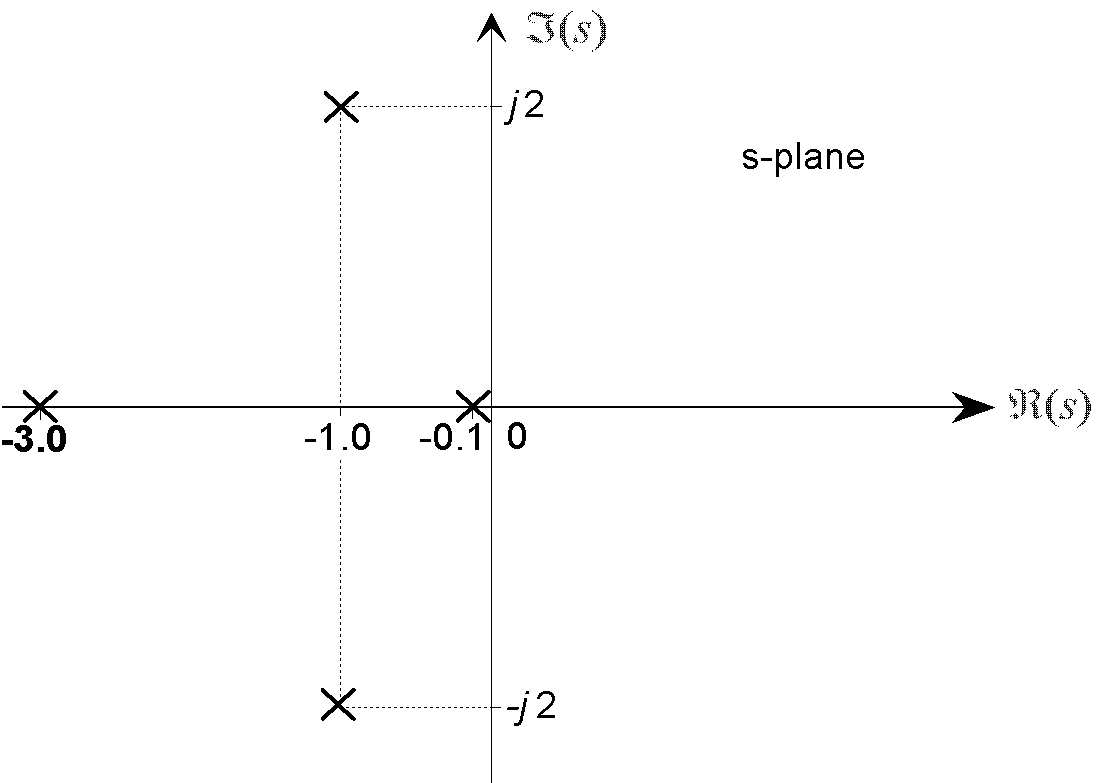
\includegraphics[scale=0.2]{img/figura3.png}
    \end{center}
  \end{tabular}
\end{center}
\textit{Figura 3: Grafíca de polo-cero de un sistema de cuarto orden con dos polos reales y dos polos complejo conjugados}
\begin{center}
  \begin{tabular}{p{16cm}}
    \textbf{Solución:} El sistema tiene cuatro polos y ningún cero. Los dos polos reales corresponden a una descomposición exponencial en terminos de $C{\scriptscriptstyle 1}e^{-3t}$ y $C{\scriptscriptstyle 2}e^{-0-1t}$ y el par de polos complejo conjugados introduce un componente oscilatorio $Ae^{-t}\sin(2t+\phi)$, de modo que el total homogéneo a la respuesta es:\\
    \begin{center}
      \begin{center}
        \[y{\scriptscriptstyle h}(t)=C{\scriptscriptstyle 1}e^{-3t}+C{\scriptscriptstyle 2}e^{-0-1t}+Ae^{-t}\sin(2t+\phi)\]
      \end{center}
      \begin{minipage}{0.9\textwidth}
        \begin{flushright}
            (12)
        \end{flushright}
      \end{minipage}
    \end{center}
    \\
    Aunque se determina las fortalezas relativas de los componentes en cualquier situación determinada por el conjunto de condiciones iniciales, se pueden hacer las siguientes observaciones generales:
    \begin{enumerate}
      \item El termino $e^{-3t}$, con una constante de tiempo $\tau$ de $0.33$ segundos, la descompone rapidamente y es significativa solo por aproximación a $4\tau$ o $1.33$ segundos.
      \item La respuesta tiene un componente oscilatorio $Ae^{-t}\sin(2t+\phi)$ definido por el par de complejos conjugados, y exhibe algún sobreimpulso. La oscilación se descompondra en aproximadamente $4$ segundos porque el termino  amortiguador $e^{-t}$.
      \item El termino $e^{-0.1t}$, con una constante de tiempo $\tau=10$ segundos, persistira aproximadamente por $40$ segundos. Por lo tanto es el componente dominante a largo plazo en la respuesta homogénea.
    \end{enumerate}
    \\\hline
  \end{tabular}
\end{center}
\clearpage
\begin{center}
  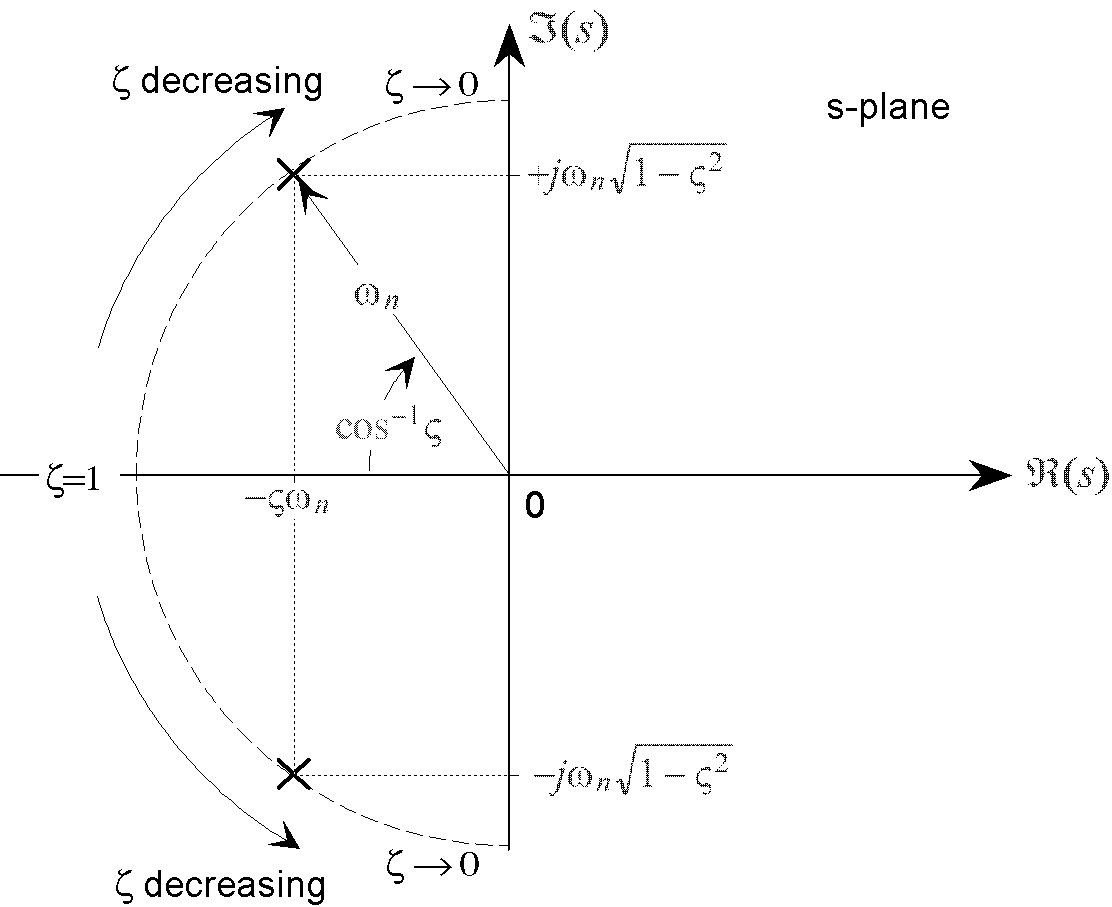
\includegraphics[scale=0.2]{img/figura4.png}
\end{center}
\textit{Figura 4: Definición de los parametros $\omega{\scriptscriptstyle n}$ y $\zeta$ para un sistema de segundo orden amortiguado de la localización polos complejo conjugados.}
La localización de polos de segundo orden en el sistema homogéneo clasico
\begin{center}
  \[\frac{d^{2}y}{dt^{2}}+2\zeta\omega{\scriptscriptstyle n}\frac{dy}{dt}+\omega^{2}{\scriptscriptstyle n}y=0\]
  \begin{minipage}{0.9\textwidth}
    \begin{flushright}
        (13)
    \end{flushright}
  \end{minipage}
\end{center}
descrito en Sección 9.3 esta dada por

\begin{center}
  \[p{\scriptscriptstyle 1},p{\scriptscriptstyle 2}=-\zeta\omega{\scriptscriptstyle n}\pm\omega{\scriptscriptstyle n}\sqrt{\zeta^{2}-1}\]
  \begin{minipage}{0.9\textwidth}
    \begin{flushright}
        (14)
    \end{flushright}
  \end{minipage}
\end{center}

Si $\zeta \geq 1$, corresponde a un sistema de amortiguamiento, de dos polos reales y encuentran en la mitad izquierda del plano. Para un sistema de amortiguamiento, $0 \leq \zeta \leq 1$, la forma del par de polos complejo conjugados,

\begin{center}
  \[p{\scriptscriptstyle 1},p{\scriptscriptstyle 2}=-\zeta\omega{\scriptscriptstyle n}\pm j\omega{\scriptscriptstyle n}\sqrt{1-\zeta^{2}}\]
  \begin{minipage}{0.9\textwidth}
    \begin{flushright}
        (15)
    \end{flushright}
  \end{minipage}
\end{center}
y estan localizados en la mitad izquierda del plano, como se muestra en la \textit{Figura 4}. Donde esta figura puede ser vista como polos que encuentran a una distancia $\omega{\scriptscriptstyle n}$ del origen, y con un angulo $\pm\cos^{-1}(\zeta)$ desde el eje real negativo.\\
Por lo tanto, los polos con un sistema de subamortiguamiento de segundo orden se encuentran en un semicirculo con un radio definido por $\omega{\scriptscriptstyle n}$, en un angulo definido por el valor de relación de amortiguamiento $\zeta$.
\subsubsection{Estabilidad del Sistema}
La estabilidad de un sistema lineal puede ser determinado directamente por la función de transferencia. Un n-esimo orden del sistema lineal es asintóticamente estable solo si todas las componentes en la respuesta homogénea de un conjunto finito se descompone a cero conforme el tiempo incrementa, o
\begin{center}
  \[ \lim_{t \to \infty} \sum_{i=1}^n C{\scriptscriptstyle i}e^{p{\scriptscriptstyle i}t}=0\]
  \begin{minipage}{0.9\textwidth}
    \begin{flushright}
        (16)
    \end{flushright}
  \end{minipage}
\end{center}
donde el $p{\scriptscriptstyle i}$ son los polos del sistema. En un sistema estable todos los componentes de la respuesta homogénea deben descomponerse a cero conforme el tiempo incremente. Si algún polo tiene una parte real positiva en un componente de salida este incrementa sin ningún límite, causando que el sistema sea inestable.
\begin{center}
  \begin{tabular}{p{16cm}}
    En orden del sistema lineal para ser estable, todos sus polos deben tener partes reales negativas, es decir todos deben estar dentro de la mitad izquierda del plano-s. Un polo "inestable", esta en la mitad derecha del plano-s, generando una respuesta al sistema homogéneo que incrementa, sin limite de alguna condición inicial finita. Un sistema tiene un o más polos que estan en el eje imaginario del plano-s tiene un oscilador que no se descompone en esta respuesta homogénea, y es definida como marginalmente estable
  \end{tabular}
\end{center}
\section{Evaluación geometrica de la Función de Transferencia}
La función de transferencia puede ser evaluada de por cualquier valor de $s=\sigma+j\omega$, y en general, cuando s es complejo la función $H(s)$ por si misma es compleja. Es trivial expresar este valor complejo de la función de transferencia en forma polar como magnitud y un angulo
\begin{center}
  \[H(s)=|H(s)|e^{j\phi(s)}\]
  \begin{minipage}{0.9\textwidth}
    \begin{flushright}
        (17)
    \end{flushright}
  \end{minipage}
\end{center}
con una magnitud $|H(s)|$ y un angulo $\phi(s)$ dado por
\begin{center}
  \[|H(s)|=\sqrt{ \mathbb{R}\{H(s)\}^{2}+ \mathbb{I}\{H(s)\}^{2}}\]
  \begin{minipage}{0.9\textwidth}
    \begin{flushright}
        (18)
    \end{flushright}
  \end{minipage}
  \\
  \[\phi(s)=\tan^{-1}\left(\frac{\mathbb{I}\{H(s)\}}{\mathbb{R}\{H(s)\}}\right)\]
  \begin{minipage}{0.9\textwidth}
    \begin{flushright}
        (19)
    \end{flushright}
  \end{minipage}
\end{center}
donde $\mathbb{R}\{\}$ es el operador real, y $\mathbb{I}\{\}$ es el operador imaginario. Si el polinomio del numerador y denominador son factorizados en terminos $(s-p{\scriptscriptstyle i})$ y $(s-z{\scriptscriptstyle i})$ como en la ecuación $(2)$
\begin{center}
  \[H(s)=K\frac{(s-z{\scriptscriptstyle 1})(s-z{\scriptscriptstyle 2})\cdots(s-z{\scriptscriptstyle m-1})(s-z{\scriptscriptstyle m})}{(s-p{\scriptscriptstyle 1})(s-p{\scriptscriptstyle 2})\cdots(s-p{\scriptscriptstyle m-1})(s-p{\scriptscriptstyle m})}\]
  \begin{minipage}{0.9\textwidth}
    \begin{flushright}
        (20)
    \end{flushright}
  \end{minipage}
\end{center}
cada uno de los factores en el numerador y del denominador son cantidades complejas, y pueden ser interpretadas como un vector en el plano-s originados por el punto $z{\scriptscriptstyle i}$ o $p{\scriptscriptstyle i}$ y directamente por $s$ que es la función que debe ser evaluada. Cada uno de estos vectores puede ser escrito en forma polar en terminos de la magnitud y un angulo, por ejemplo para el polo $p{\scriptscriptstyle i}=\sigma{\scriptscriptstyle i} + \omega{\scriptscriptstyle i}$, la magnitud y angulo del vectir para el punto $s=\sigma + \omega$ es
\begin{center}
  \[|s-p{\scriptscriptstyle i}|=\sqrt{(\sigma-\sigma{\scriptscriptstyle i})^2+(\omega-\omega{\scriptscriptstyle i})^2}\]
  \begin{minipage}{0.9\textwidth}
    \begin{flushright}
        (21)
    \end{flushright}
  \end{minipage}
  \\
  \[\angle (s-p{\scriptscriptstyle i}) = \tan^{-1}\left(\frac{\omega-\omega{\scriptscriptstyle i}}{\sigma-\sigma{\scriptscriptstyle i}}\right)\]
  \begin{minipage}{0.9\textwidth}
    \begin{flushright}
        (22)
    \end{flushright}
  \end{minipage}
\end{center}

como se muestra en la \textit{Figura 5(a)}. Porque la magnitud de el producto dos cantidades complejas es el producto individual de sus magnitudes, y el angulo es el producto de la suma de los angulos (Anpéndice B), la magnitud y el angulo completo de la función de transferencia puede ser entonces escrito como

\begin{center}
  \[|H(s)|=K\frac{\prod_{i=1}^m |(s-z{\scriptscriptstyle i})|}{\prod_{i=1}^n |(s-p{\scriptscriptstyle i})|}\]
  \begin{minipage}{0.9\textwidth}
    \begin{flushright}
        (23)
    \end{flushright}
  \end{minipage}
  \\
  \[\angle H(s) = \sum_{i=1}^m \angle(s-z{\scriptscriptstyle i}) - \sum_{i=1}^n \angle(s-p{\scriptscriptstyle i})\]
  \begin{minipage}{0.9\textwidth}
    \begin{flushright}
        (24)
    \end{flushright}
  \end{minipage}
\end{center}
La magnitud de cada uno de los vectores componentes en el numerador y denominador es la distancia del punto $s$ desde el polo o cero en el plano-s. Por lo tantom si el vector desde el polo $p{\scriptscriptstyle i}$ a el punto $s$ en la grafíca polo-cero tiene una longitud $q{\scriptscriptstyle i}$ y un angulo $\theta{\scriptscriptstyle i}$ desde la horizontal, y el vector desde
\clearpage
\begin{center}
  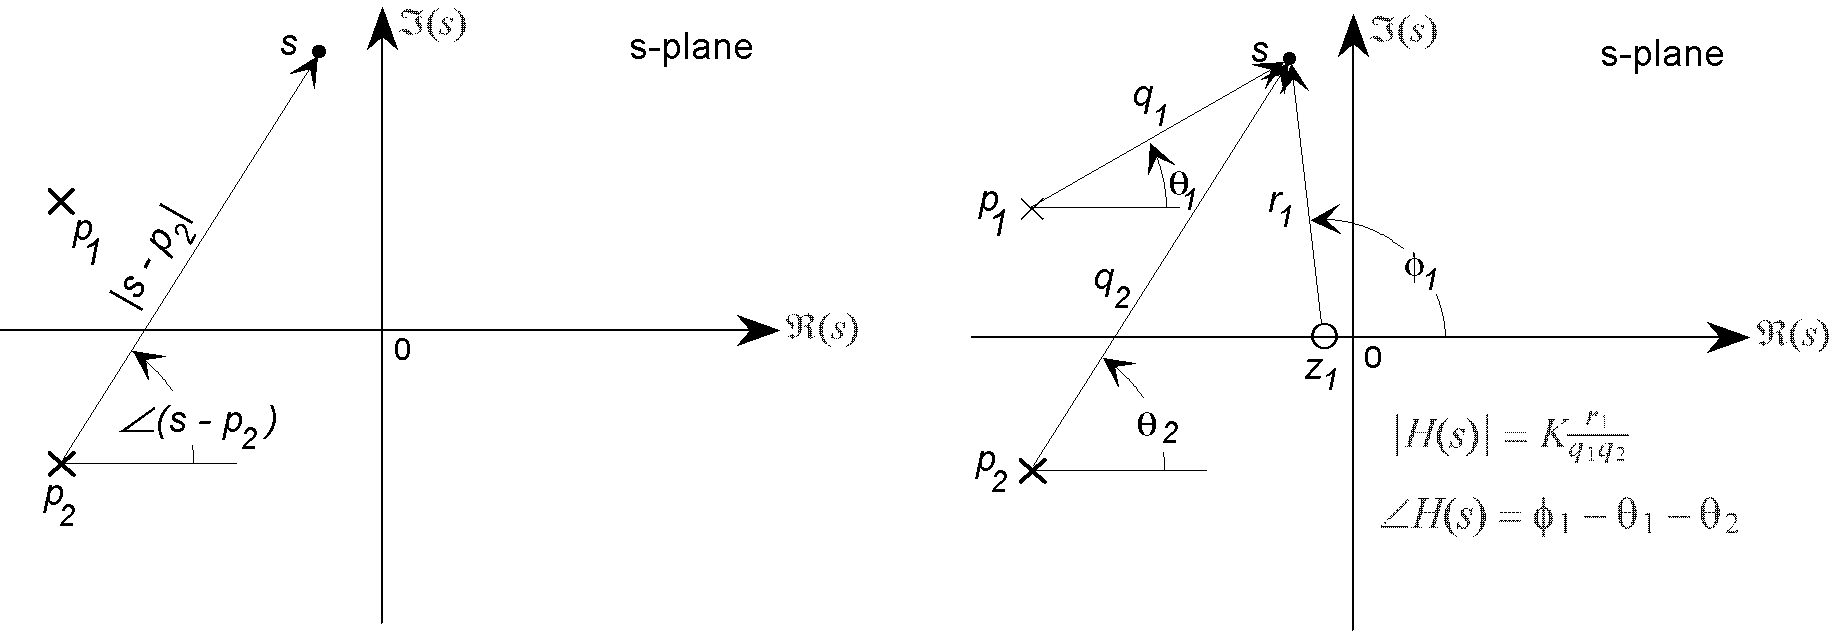
\includegraphics[scale=0.2]{img/figura5a.png}
\end{center}
\textit{Figura 5: (a) Definición geometrica en forma polar en el plano-s. (b) Evaluación geometrica de la función de transferencia en la grafíca polo-cero.}\\
\vspace{0.25cm}el cero $z{\scriptscriptstyle i}$ a el punto $s$ tiene una longitud $r{\scriptscriptstyle i}$ y un angulo $\phi{\scriptscriptstyle i}$, como se muestra en la \textit{Figura 5(b)}, el valor de la función de transferencia en el punto $s$ es
\begin{center}
  \begin{minipage}{0.9\textwidth}
    \[|H(s)|= K \frac{r{\scriptscriptstyle 1}\cdots r{\scriptscriptstyle m}}{q{\scriptscriptstyle 1}\cdots q{\scriptscriptstyle n}}\]
    \begin{flushright}
        (25)\\
    \end{flushright}
  \end{minipage}
  \[\angle H(s)=(\phi{\scriptscriptstyle 1}+\cdots+\phi{\scriptscriptstyle m})-(\theta{\scriptscriptstyle 1}+\cdots\theta{\scriptscriptstyle n})\]
  \begin{minipage}{0.9\textwidth}
    \begin{flushright}
        (26)
    \end{flushright}
  \end{minipage}
\end{center}
Por lo tanto, la función de transferencia evaluada en alguno valor de $s$ determina la grafíca de polo-cero geometricamente, excepto el total de ganancia del factor $K$. La magnitud de la función de transferencia es proporcional al producto de las distancias geometricas del plano-s de cada uno de los ceros a el punto s dividido por el producto de las disctancias de cada uno de los polos al punto. El angulo de la función de transferencia es la suma de los angulos de los vectores asociados con los ceros menos la suma de los angulos de los vectores asociados con los polos.
\begin{center}
  \begin{tabular}{p{16cm}}
    \hline
    Ejemplo\\
    Un sistema de segundo orden tiene un par de polos complejo conjugados $s=-2\pm 3j$ y un solo cero en el origen del plano-s. Encontrar la función de transferencia y usa la grafíca de polo-cero para evaluar la función de transferencia en $s=0+5j$.\\
    \textbf{Solución: } De la descripción del problema
    \begin{center}
      \[H(s)= K \frac{s}{(s-(-2+3j))(s-(-2-3j))}\]\\
      \[=K\frac{s}{s^{2}+4s+13}\]
    \begin{minipage}{0.9\textwidth}
      \begin{flushright}
          (27)
      \end{flushright}
    \end{minipage}
    \end{center}
    La grafíca de polo-cero como se muestra en la \textit{Figura 6}. De la figura a la función de transferencia es
    \begin{center}
      \[H(s)=K\frac{\sqrt{(0-5)^{2}}}{\sqrt{(0-(-2))^{2}+(5-3)^{2}}\sqrt{(0-(-2))^{2}+(5-(-3))^{2}}}\]\\
      \[=K\frac{5}{4\sqrt{34}}\]
      \begin{minipage}{0.9\textwidth}
        \begin{flushright}
          (28)
        \end{flushright}
      \end{minipage}
    \end{center}
  \end{tabular}
\end{center}
\clearpage
\begin{center}
  \begin{tabular}{p{16cm}}
    \begin{center}
        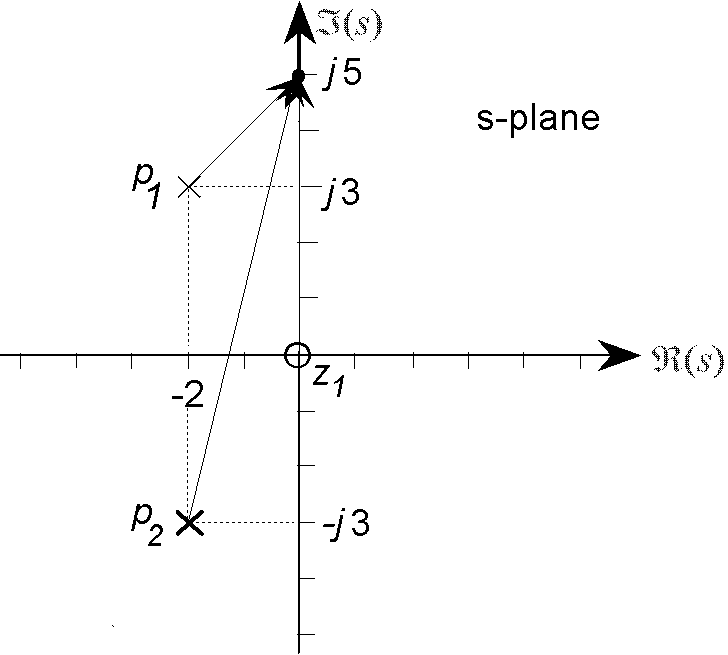
\includegraphics[scale=0.2]{img/figura6.png}\\
        \textit{Figura 6: Grafíca de polo-cero de un sistema de segundo orden con un cero en el origen}
    \end{center}
    Y
    \begin{center}
      \[\angle H(s)= \tan^{-1}(5/0)-\tan^{-1}(2/2)-\tan^{-1}(8/2)\]\\
      \[=-31^{\circ}\]
      \begin{minipage}{0.9\textwidth}
        \begin{flushright}
          (29)
        \end{flushright}
      \end{minipage}
    \end{center}
    \\\hline
  \end{tabular}
\end{center}
\section{Respuesta en frecuencia y la grafíca de polos-ceros}
La respues en frecuencia puede ser escrita en terminos del sistema de polos y ceros sustituyendo $j\omega$ por s directamente dentro de la forma factorizada de la función de transferencia:
\begin{center}
  \[H(j\omega)=K \frac{(j\omega-z{\scriptscriptstyle 1})(j\omega-z{\scriptscriptstyle 2})\cdots(j\omega-z{\scriptscriptstyle m-1})(j\omega-z{\scriptscriptstyle m})}{(j\omega-p{\scriptscriptstyle 1})(j\omega -p{\scriptscriptstyle 2})\cdots(j\omega -p{\scriptscriptstyle m-1})(j\omega -p{\scriptscriptstyle m})}\]
  \begin{minipage}{0.9\textwidth}
    \begin{flushright}
      (30)
    \end{flushright}
  \end{minipage}
\end{center}
Porque la respuesta en frecuencia es la función de transferencia evaluada en el eje imaginario del plano-s, cuando $s=j\omega$, descrito por la evaluación sobre el método grafíco en la función de transferencia puede ser aplicado directamente a la respuesta en frecuencia. Cada uno de los vectores n-esimo del sistema de polos puede ser $s=j\omega$ que tiene una magnitud y un angulo:
\begin{center}
  \[|j\omega-p{\scriptscriptstyle i}| = \sqrt{\sigma^2{\scriptscriptstyle i}+(\omega-\omega{\scriptscriptstyle i})^2}\]
  \begin{minipage}{0.9\textwidth}
    \begin{flushright}
      (31)
    \end{flushright}
  \end{minipage}
  \[\angle(j\omega-p{\scriptscriptstyle i})= \tan^{-1}\left(\frac{\omega-\omega{\scriptscriptstyle i}}{-\sigma{\scriptscriptstyle i}}\right)\]
  \begin{minipage}{0.9\textwidth}
    \begin{flushright}
      (32)
    \end{flushright}
  \end{minipage}
\end{center}
así como se muestra en la \textit{Figura 7}, con expresiones similares para los vectores de $m$ ceros. La magnitud y fase del angulo del complemento a la respuesta en frecuencia puede ser escrita en terminos de las magnitudes y angulos de esos vectores
\begin{center}
  \[|H(j\omega)|=K\frac{\prod_{i=1}^m |(j\omega-z{\scriptscriptstyle i})|}{\prod_{i=1}^n |(j\omega-p{\scriptscriptstyle i})|}\]
  \begin{minipage}{0.9\textwidth}
    \begin{flushright}
      (33)
    \end{flushright}
  \end{minipage}
  \[\angle H(j\omega) = \sum_{i=1}^m \angle(j\omega-z{\scriptscriptstyle i}) - \sum_{i=1}^n \angle(j\omega-p{\scriptscriptstyle i})\]
  \begin{minipage}{0.9\textwidth}
    \begin{flushright}
      (34)
    \end{flushright}
  \end{minipage}
\end{center}
\clearpage
\begin{center}
  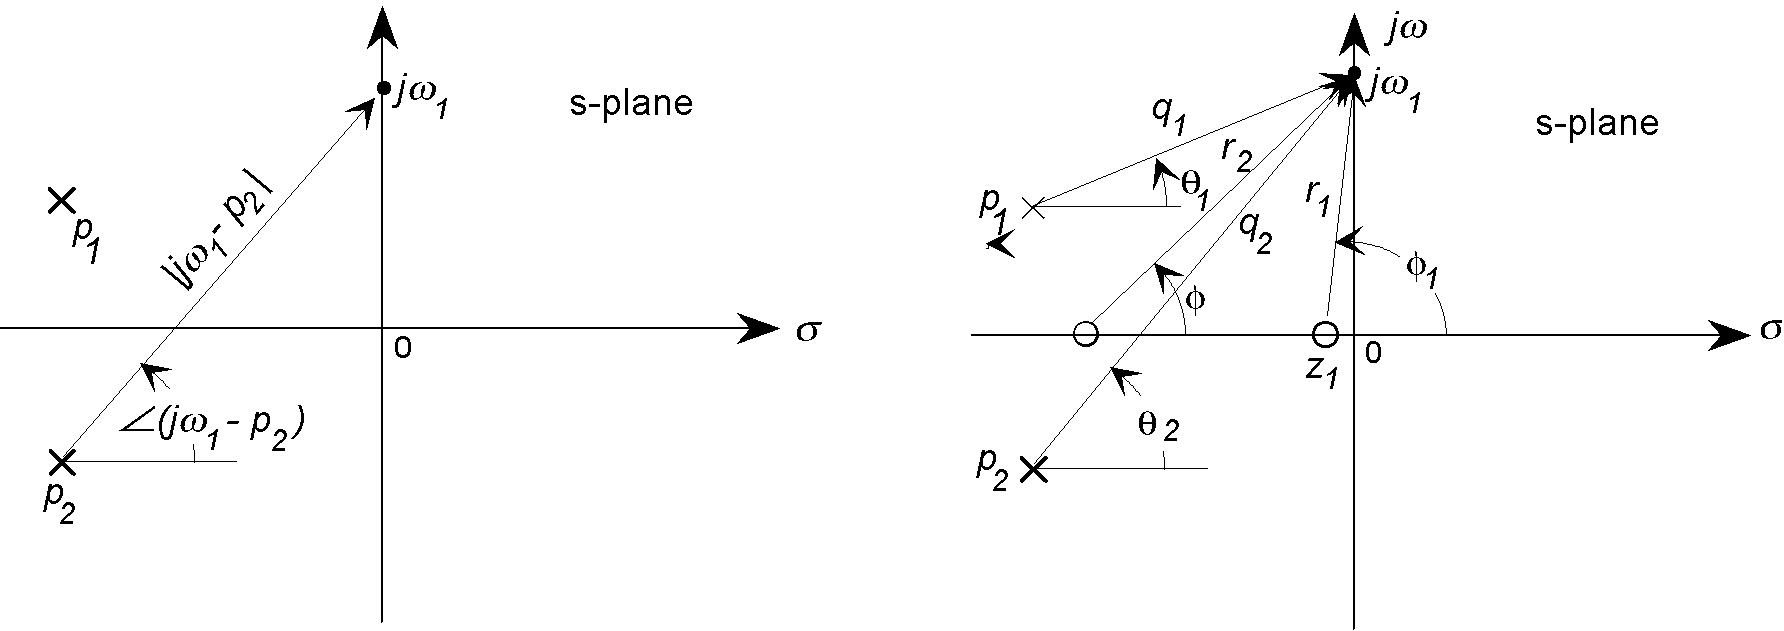
\includegraphics[scale=0.25]{img/figura7.png}
\end{center}
\textit{Figura 7: Definición de las cantidades vectoriales usando en las definiciones función de respuesta en frecuencia de la grafíca de polo-cero. En (a) el vector del polo (o cero) es definido, en (b) el vector de todos los polos y ceros en el sistema es mostrado.}
\\
\vspace{0.15cm}
Es definido sobre, si el vector del polo $p{\scriptscriptstyle i}$ a el punto $s=j\omega$ tiene una longitud $q{\scriptscriptstyle i}$ y un angulo $\omega{\scriptscriptstyle i}$ de la horizontal, y el vector de los ceros $z{\scriptscriptstyle i}$ al punto $j\omega$ tiene una longitud $r{\scriptscriptstyle i}$ y un angulo $\phi{\scriptscriptstyle i}$,, como se muestra en la \textit{Figura 7b}, el valor de la respuesta en frecuencia en el punto $j\omega$ es
\begin{center}
  \[|H(j\omega)|=K\frac{r{\scriptscriptstyle 1}\cdots r{\scriptscriptstyle m}}{q{\scriptscriptstyle 1}\cdots q{\scriptscriptstyle m}}\]
  \begin{minipage}{0.9\textwidth}
    \begin{flushright}
      (35)
    \end{flushright}
  \end{minipage}
  \[\angle H(j\omega)=(\phi{\scriptscriptstyle 1}+\cdots +\phi{\scriptscriptstyle m})-(\theta{\scriptscriptstyle 1}+\cdots +\theta{\scriptscriptstyle m})\]
  \begin{minipage}{0.9\textwidth}
    \begin{flushright}
      (36)
    \end{flushright}
  \end{minipage}
\end{center}
El método grafíco puede ser muy util para derivar imagenes de forma cualitativa del sistema de respuesta en frecuencia. Por ejemplo, cosiderar una respuesta sinusoidal en un sistema de primer orden con un polo en el eje real $s=\frac{-1}{\tau}$ como se muestra en la \textit{Figura 8a}, y la grafíca de Bode en la \textit{Figura 8b}. A si mismo pensamos que la constante $K$ de ganancia no puede estar determinada por la grafíca de polo-cero, las siguientes observaciones debe estar hecha directamente por debajo de la magnitud y el angulo del vector desde el polo al eje imaginario como la entrada variada de frecuencia:
\begin{enumerate}
  \item Para bajas frecuencias la ganancia se aproxima a un valor finito, y la fase del angulo tiene un pequeño y finito retraso.
  \item Mientras que la frecuencia de entrada incrementa la ganancia decrece (porque la longitud del vector incrementa), y el retrasa de la fase tambien incrementa (el angulo del vector se alarga).
  \item Para las altas frecuencias de entrada la ganancia se aproxima a cero, y la fase del angulo se aproxima a $\pi /2$
\end{enumerate}
Para el segundo ejemplo se considera un sistema de segundo orden, con la relación de amortiguación se escogen un por de complejos conjugados que estan localizados cerca del eje imaginario  como se muestra en la \textit{Figura 9a}. En este caso hay un par de vectores conectados por dos polos al eje imaginario, y la consiguiente conclusión puede ser dibujada por como las longitudes y angulos de los vectores cambia conforme la frecuencia recorre el eje imaginario:
\begin{enumerate}
  \item Para bajas frecuencias hay una ganancia finita (pero indeterminada) y una pequeña pero un sistema de retraso asociado a una fase finita.
  \item Para la el incremento de la frecuencia de entrada y el punto de prueba en el eje imaginario se aproxima al polo, uno de los vectores (asociado con el polo en el segundo cuadrante) decrementa en longitud
  \clearpage
  \begin{center}
    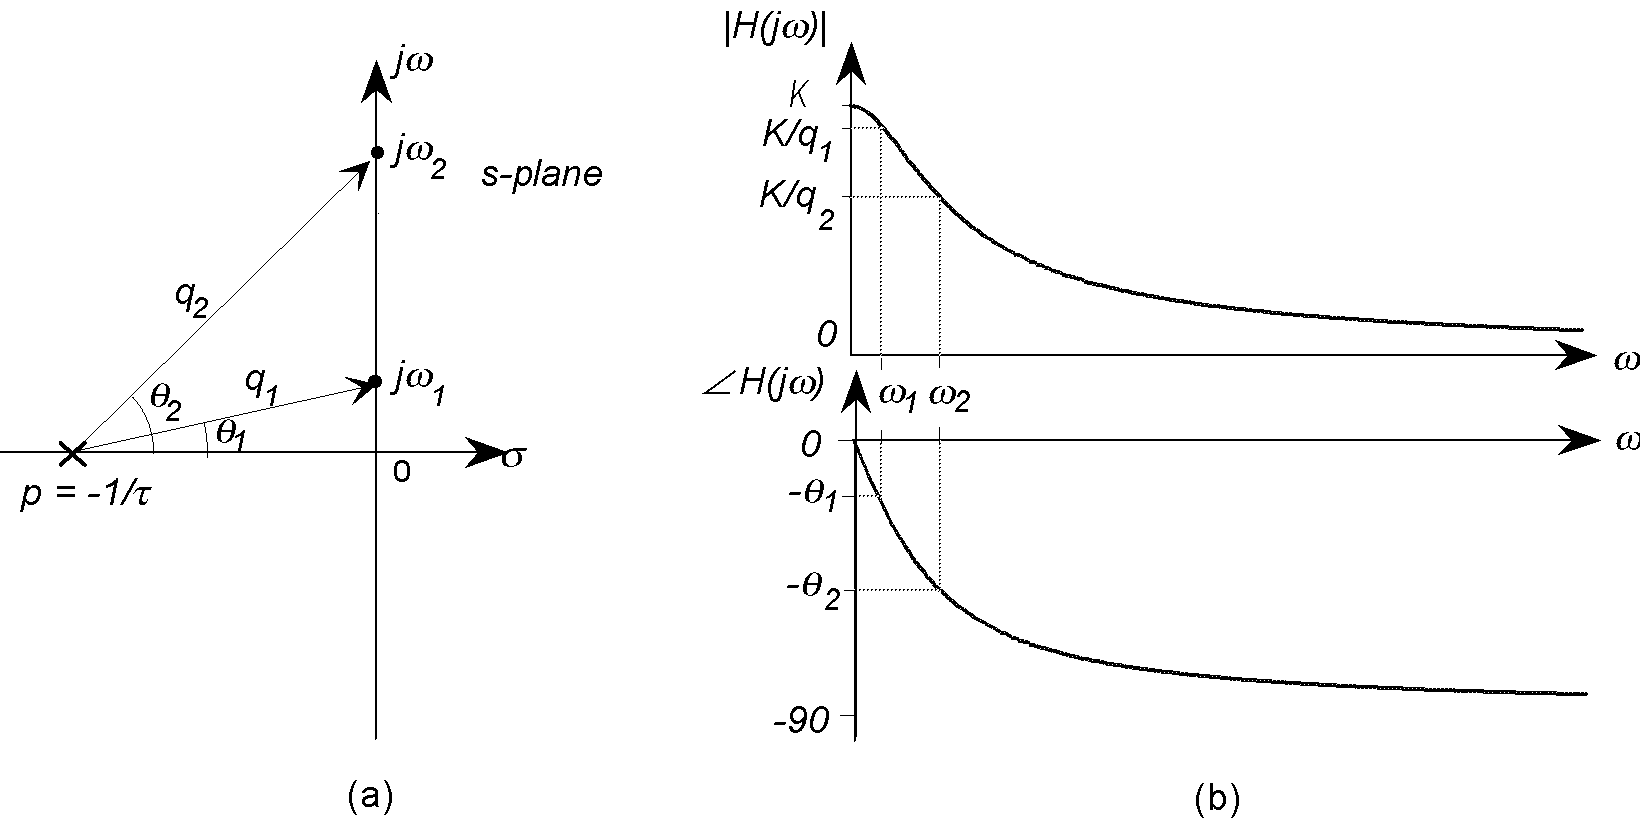
\includegraphics[scale=0.25]{img/figura8.png}
  \end{center}
  \textit{Figura 8: Grafíca de polo-cero de un sistema de primer orden y con la función de respuesta en frecuencia}\\
  \vspace{0.25cm}
  y algunos puntos se alargan a un minimo. Hay un incremento en el valor de la función de magnitud sobre el rango de la frecuencia cerrada al polo
  \item Para frecuencias muy altas, la longitud de ambos vectores tiende a infinito, y la magnitud de la respuesta en frecuencia tiende a cero, mientras la fase se aproxima a un angulo de $\pi$ radianes porque el angulo de cada vector se aproxima a $\pi/2$
\end{enumerate}
Las siguientes generalizaciones pueden ser acerca de la frecuencia de respuesta de un sistema sinusoidal lineal, basandose en la interpretación geometrica de la grafíca polo-cero:
\begin{enumerate}
  \item Si un sistema tiene un exceso de polos sobre el número de ceros, la magnitud de la respuesta en frecuencia sera larga. Similarmente, si un sistema excede el número de ceros la ganancia incrementara sin limite, ya que la frecuencia de entrada incrementa. Eso no puede pasar en sistemas de energía física porque implicaria una ganancia de potencia infinita sobre el sistema.
  \item Si el sistema tiene un par de polos complejo conjugados cerca del eje imaginario, la magnitud de la respuesta en frecuentcia tendra un pico, o resonancia en la proximidad del polo en frecuencia. Si el par de polos se encuentran directamente sobre el eje imaginario, el sistema exhibira una ganancia infinita en frecuencia.
  \item Si el sistema tiene un par de ceros conjugados cerca de el eje imaginario, la respuesta en frecuencia tendra un inclinación o muesca en su función de magnitud en frecuencia en la cercania del cero. Los par de ceros deben encontrarse directamente sobre el eje imaginario, la respuesta es identica a cero en la frecuencia de cero, y el sistema no respondera a todas las exitaciones sinusoidales de la frecuencia
  \item Un polo en el origen del plano-s (correspodera a una integración de terminos pura en la función de transferencia) implicara una ganancia infinita de frecuencia cero.
  \item Similarmente al cero en el origen del plano-s (correspondera a una diferenciación pura) implica una ganancia cero para el sistema de frecuencia cero.
\end{enumerate}
\clearpage
\begin{center}
  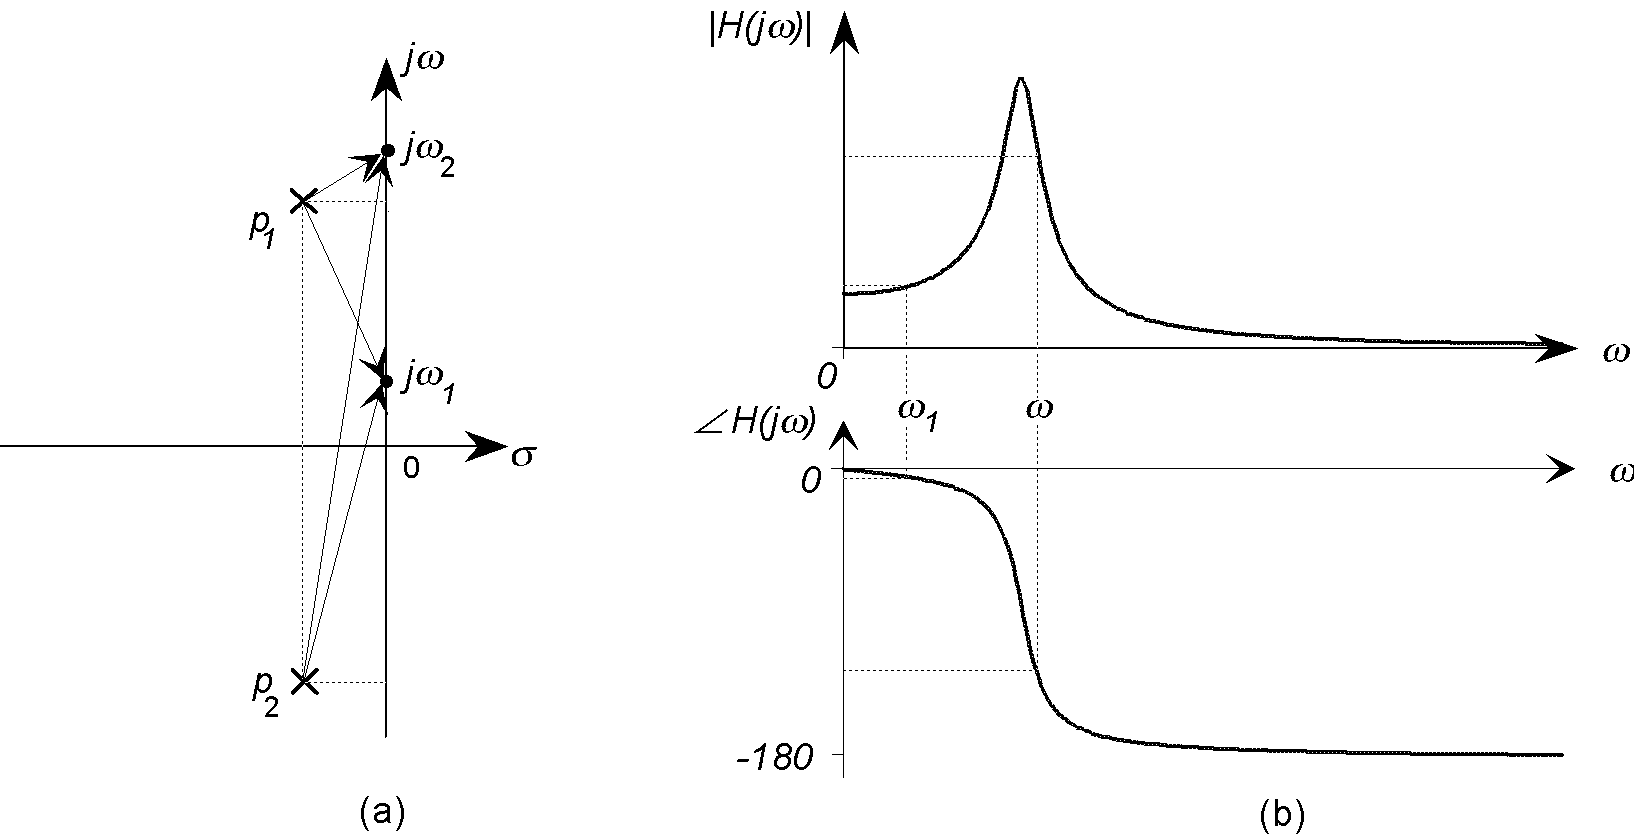
\includegraphics[scale=0.25]{img/figura9.png}
\end{center}
\textit{Figura 9: La grafíca de polo-cero de un sistema de segundo orden y es la función de respuesta de esa frecuencia.}
\subsection{Un Método Simple para construcción de la Grafíca de Magnitud Bode directamente de la Grafíca de Polo-Cero}
Las graficas de polo-cero de un sistema contiene suficiente informacion que define la respuesta en frecuencia excepto por una ganancia constante arbitraría. Es frecuentemente suficiente saber la forma de la frecuencia de la grafíca de Bode sin conocer la ganancia absoluta. El metodo describe aqui la grafíca de magnitud de permitancia sera bosquejada por inspección, sin dibujar las curvas individuales del componente. El método es basado en el hecho de que todas las curvas de magnitud  generales sufren un cambio en la pendiente de frecuencia de corte.\\
El primer paso es identificar la frecuencia de corte, ambas son factores de la función de transferencia o directamente de la grafíca de polo-cero, Codiderando una grafíca polo-cero tipíca de un sistema lineal como se muestra en la \textit{Figura 10a}. La frecuencia de corte para los cuatro bloques de primer y segundo orden estan todas en una frecuencia igual a la distancia radial de los polos o ceros desde el origen del plano-s, es $\omega{\scriptscriptstyle b}=\sqrt{\sigma^{2}+\omega^{2}}$.
Por lo tanto, todas las frecuencias de corte deben ser encontradas tomando un compas y dibujando un arco sobre cada polo o cero hacía el eje positivo imaginario. Esas frecuencias de corte pueden ser directamente tranferidas a la frecuencia logaritmica de la grafíca de Bode.\\
Porque todas las frecuencias bajas asintóticas son lineas horizontales con una ganancia de $0dB$, un polo o cero no debe contribuir a la magnitud grafíca de Bode por debajo de la frecuencia de corte. Cada uno de los polos o ceros contribuye a cambiar en la inclinación de la grafíca asintótica de $\pm20dB$/decada sobre la frecuencia de corte. Un par de polos o ceros complejo conjugados define dos coincidentes cortes de $\pm20dB$/decada (una para cada miembro del par), dando un total de cambios en la inclinación de $\pm40dB$/decada. Por lo tanto,para alguna frecuencia $\omega$, la inclinación de la función de magnitud asintótica depende solo en el número de puntos de corte en la frecuencia baja a $\omega$, o para la izquierda de la grafíca de Bode. Si hay $Z$ puntos de corte debido a ceros de la izquierda, y $P$ puntos de corte debido a los polos, la pendiente de frecuencia en la curva es  $20\times(Z-P)db/decada$.\\
Algunos polos o ceros en el origen no pueden ser graficados en la grafíca de Bode, porque estan efectivamente a la izquierda de todas las finitas frecuencias de cortes. Sin embargo, la define la inclinación incial. Si una frecuencia inicial arbitraría y una ganancia asumida (por ejemplo $0dB$) en esa frecuencia son escogidas, el trazo de la grafíca de la magnitud puede ser facilmente construida por ninguna inclinación inicial, y construida por
\begin{center}
  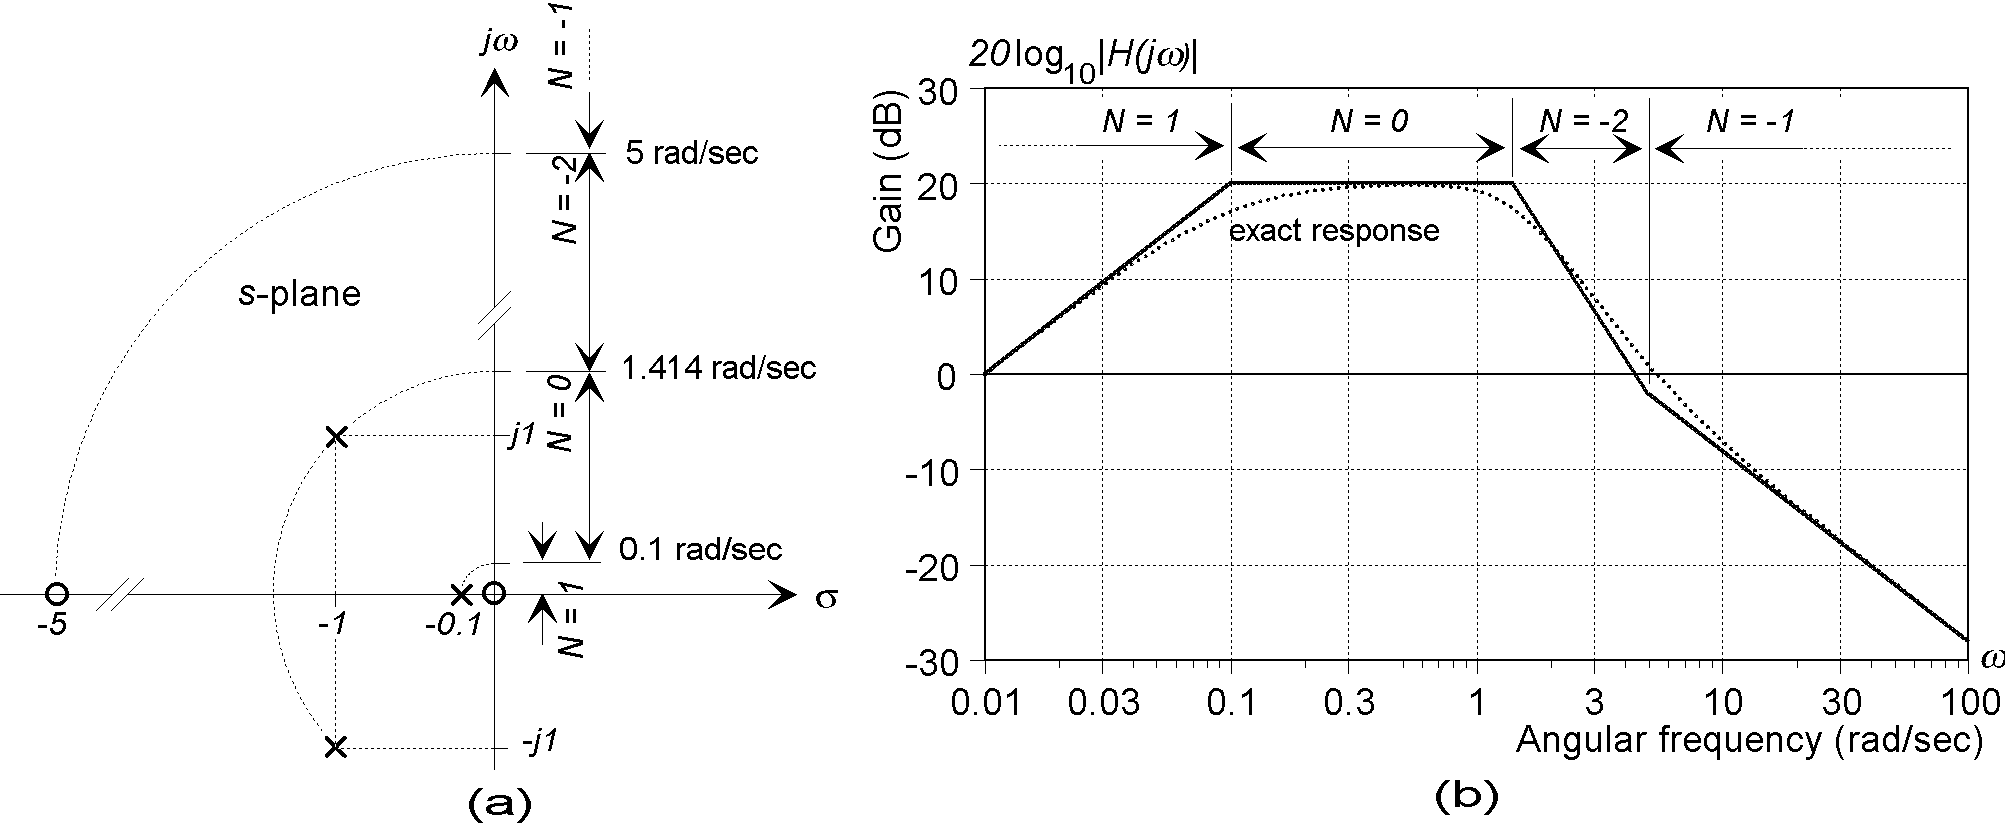
\includegraphics[scale=0.25]{img/figura10.png}
\end{center}
\textit{Figura 10: Construcción de la grafíca de magnitud de Bode desde el diagrama de polo-cero: (a) muestra un sistema de tercer orden tipíco, y la definición de la frecuencia de corte, (b) muestra la grafíca de Bode basada en los cambios de inclinación de las frecuencias de corte}\\
\vspace{0.25cm}
curvas desde el segmendo recto que cambia en la inclinación de unidades de $\pm20dB$/decada en el punto de corte. La selección arbitraría de referencia la ganacia resulta en un desplazamiento vertical a la curva.\\
La \textit{Figura 10b} muesta la magnitud grafíca del plano del sistema que se muestra en la \textit{Figura 10a} construida usando este metodo. Un rango de frecuencia de $0.01$ a $100 radianes/segundo$ eran selecciones arbitrarias, y una ganancia de $0dB$ a $0.01 radianes/segundo$ fue designada como nivel de referencia. Las frecuencias de corte de $0$, $0.1$, $1.414$, y $5 radianes/segundo$ fueron transferidas al eje de la frecuencia de la grafíca de polo-cero. El valor de $n$ en alguna frecuencia es $Z-P$, donde $Z$ es el número de ceros a la izquierda, y $P$ es el número de polos a la izquierda. La curva esta simplificamente dibujada por asignación del valor de la inclinación de cada una de los intervalos de frecuencia y se dibujan lineas que lo conectan.
\end{document}
